%%%%%%%%%%%%%%%%%%%%%%%%%%%%%%%%%%%%%%%%%%%%%%%%%%%%%%%%%%%%%%%%%%%%%%%%%%%
%
% Plantilla para un artículo en LaTeX en español.
%
%%%%%%%%%%%%%%%%%%%%%%%%%%%%%%%%%%%%%%%%%%%%%%%%%%%%%%%%%%%%%%%%%%%%%%%%%%%

% Qué tipo de documento estamos por comenzar:
\documentclass[a4paper]{article}
% Esto es para que el LaTeX sepa que el texto está en español:
\usepackage[spanish]{babel}
\selectlanguage{spanish}
% Esto es para poder escribir acentos directamente:
\usepackage[utf8]{inputenc}
\usepackage[T1]{fontenc}



%% Asigna un tamaño a la hoja y los márgenes
\usepackage[a4paper,top=3cm,bottom=2cm,left=3cm,right=3cm,marginparwidth=1.75cm]{geometry}

%% Paquetes de la AMS
\usepackage{amsmath, amsthm, amsfonts}
%% Para añadir archivos con extensión pdf, jpg, png or tif
\usepackage{graphicx}
\usepackage[colorinlistoftodos]{todonotes}
\usepackage[colorlinks=true, allcolors=blue]{hyperref}

%% Primero escribimos el título
\title{Impacto en el PIB después de la pandemia de COVID-19 en México}
\author{Edgar Ramírez González\\ Mariana Garfias Martínez\\ Rodrigo Bertheau Rangel\\
  \small Benemérita Universidad Autónoma de Puebla\\
  \small edgargz777@gmail.com\\
  \small ms.marianagarfias@gmail.com\\
  \small rodrigobertheau88@gmail.com\\
  \small Registro Académico y Científico del Español
  \date{}
}

%% Después del "preámbulo", podemos empezar el documento

\begin{document}
%% Hay que decirle que incluya el título en el documento
\maketitle

%% Aquí podemos añadir un resumen del trabajo (o del artículo en su caso) 
\begin{abstract}
Vamos a obtener mediante un enfoque econométrico un pronóstico del PIB de México con el efecto COVID-19 sobre los indicadores originales que consideramos los más afectados. Esta estimación se realiza bajo los supuestos de regresión por mínimos cuadrados ordinarios ya que nos permite ver el comportamiento de las variables de manera independiente en el modelo para tener un mejor entendimiento del resultado obtenido y un análisis fuerte del indicador.  
\end{abstract}

% Keywords command
\providecommand{\keywords}[1]
{
  \small	
  \textbf{\textit{Palabras clave: }} #1
}
\keywords{PIB, estimación, economía, COVID-19, regresión, pronostico}

%% Iniciamos "secciones" que servirán como subtítulos
%% Nota que hay otra manera de añadir acentos
\section{Introducci\'on}

Obtener un pronóstico acerca del futuro económico de un país, involucra observar el pasado para visualizar el futuro, sin embargo, toda estimación es afectada cuando se presenta una variable no contemplada, como la pandemia de COVID-19, e influye de manera directa o indirecta en la mayoría de los sectores en juego.

La Organización Mundial del Comercio, según reporta El Economista, ha pronosticado una caída del 6.6\% en el PIB del país principalmente debido a la pandemia, sin embargo, también se señalan factores internos de inversión. Así mismo, Expansión advierte que podría haber una mayor caída debido a la dependencia del país a las inversiones y comercio internacional, según analistas privados en una encuesta llevada a cabo por el banco central. Las publicaciones anteriores dan pronósticos para el cierre de año, sin dar resultados inmediatos para los primeros trimestres, pudiendo resultar menos objetivos para el estudio del PIB específicamente después de la pandemia.

El objetivo de este proyecto es predecir mediante un enfoque econométrico el PIB de México con este nuevo efecto sobre los indicadores originales que consideramos los más afectados. La razón de dicho análisis surge a partir de la suposición de que, con las medidas de salubridad, la actividad económica se ve afectada, lo cual nos conduce a pensar que veremos un decrecimiento de este indicador; aunado a esto, la recesión que se avecinaba en la era pre COVID hará que los efectos de este sean especialmente notables en nuestra economía.



\section{Metodología}

Esta investigación es documental ya que para poder llegar a los objetivos se necesita información histórica. Se consultaron 13 fuentes informativas y 8 bases de datos, dentro de todo esto se encontraban blogs personales, páginas oficiales del gobierno y artículos de páginas oficiales, de los cuales sólo se tomaron 11. Primero fundamentándose en que las bases de datos sean únicamente provenientes de páginas oficiales del gobierno. Las fuentes informativas como revistas y periódicos digitales se verificaron por la calidad de los orígenes de sus encuestas para llegar a los pronósticos, siendo elegidos sólo los artículos que hicieron su investigación en medios reconocidos u oficiales, así como con especialistas de medios relevantes y oficiales para hablar sobre la situación actual. Otro punto esencial para la discriminación de fuentes fue la preferencia de medios informativos especializados en economía y finanzas. \cite{Banxico1} \cite{Banxico2} \cite{Expansion1} \cite{Expansion2} \cite{Economista} \cite{Forbes}
\\
\\

Para llevar a cabo esta investigación se usará el método de modelo lineal bajo estimación de mínimos cuadrados ordinarios con transformaciones logarítmicas y un indicador autorregresivo de un rezago.

Se han seleccionado un total de 6 variables para describir el PIB; estas son:

\begin{itemize}
\item   	Balanza comercial de importaciones
\item   	Balanza comercial de exportaciones

En un mundo globalizado, es importante disponer de estadísticas que permitan conocer la evolución de los principales componentes del comercio internacional de mercancías, que apoyen el diseño y evaluación de políticas públicas, la toma de decisiones de particulares y la realización de diversas investigaciones. Con el objetivo de atender esta creciente demanda de información, se presenta el valor mensual de exportaciones e importaciones de mercancías, las cuales han cumplido con la normatividad aduanera.

\item   	Indicador de la Actividad Industrial

El Indicador Mensual de la Actividad Industrial permite conocer y dar seguimiento a la evolución mensual del sector industrial. Para su cálculo se utilizan: el esquema conceptual, los criterios metodológicos, la clasificación de actividades económicas y las fuentes de información, que se emplean en los cálculos anuales y trimestrales del Producto Interno Bruto. Este cálculo se alinea con las cifras anuales utilizando la técnica Denton.

\item   	Indicador Trimestral del consumo privado en el mercado interior

El Indicador Mensual del Consumo Privado en el Mercado Interior (IMCPMI), mide la evolución del gasto realizado por los hogares en bienes y servicios de consumo, tanto de origen nacional como importado, permitiendo con ello dar seguimiento de forma mensual al componente más significativo del producto, por el lado de la demanda.

\item   	Indicador de la Inversión fija bruta

Información que permite un amplio conocimiento sobre el comportamiento de la inversión en el corto plazo, misma que está integrada por los bienes utilizados en el proceso productivo durante más de un año y que están sujetos a derechos de propiedad. Este indicador muestra cómo una gran parte del nuevo valor agregado bruto en la economía se invierte, en lugar de ser consumido.

\item   	El tipo de cambio (FIX)

Es determinado por el Banco de México con base en un promedio de cotizaciones del mercado de cambios al mayoreo para operaciones liquidables el segundo día hábil bancario siguiente y que son obtenidas de plataformas de transacción cambiaria y otros medios electrónicos con representatividad en el mercado de cambios.

\end{itemize}

Un rápido análisis de dichas variables nos hace ver la necesidad de transformar los datos a una forma logarítmica para poder reducir varianza.


\section{Resultados}

Los resultados obtenidos nos indicaron una notable desaceleración económica, la cual se venía gestando tiempo previo a la actual situación pero que se intensificó sobre todo en el sector del consumo/demanda. Nuestro intercepto negativo en la relación lineal propuesta por nuestra ecuación nos señala un promedio de -61.6 puntos en el PIB cuando la actividad industrial, el consumo en el mercado y el PIB anterior tienen un efecto nulo sobre el actual (Ceteris Paribus). \\

También, el rezago en el PIB es positivo pero su influencia en el modelo se vio opacado por su coeficiente tan cercano a cero, su mayor varianza -lo cual es lógico dado de dónde proviene- y por la diferencia que hay en la relación simbólica entre la actividad industrial (oferta) y el consumo interior (demanda).\\

Esto último nos deja claro que nuestro modelo de estimación lineal es objeto de la ley principal que rige el mercado, y que, debido al paro significativo de las actividades y labores económicas, está en una tendencia decreciente; lo cual, nos demuestra que el PIB mexicano bajo los supuestos y variables propuestas en este modelo, va desacelerando considerablemente cada de cuarentena.\\

\subsection{Análisis del PIB}

Antes de plantear un modelo de regresión lineal nos propusimos analizar al PIB para percatarnos si existe algún tipo de correlación con términos anteriores de el mismo o con las variables escogidas.

\subsection{Análisis de correlación}

Para este análisis hicimos uso del coeficiente de correlación de Pearson obteniendo así la siguiente matriz:

\begin{figure}[h]
\centering
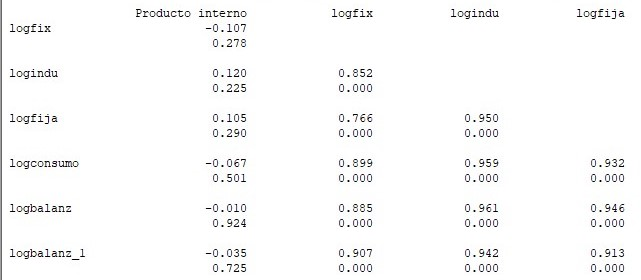
\includegraphics[width=0.7\textwidth]{6.jpg}
\caption{\label{fig:tesla}Matríz de correlación.}
\end{figure}

Es claro que no existe una correlación significativa del P de Pearson con las variables descriptivas por lo cual pueden ser utilizadas en el modelo.

\subsection{Análisis de autocorrelación}

Haciendo un análisis de autocorrelación a nuestra variable del PIB pudimos notar que hay autocorrelación en un término por lo cual vemos necesario incluir este dentro de las variables.

\begin{figure}[h]
\centering
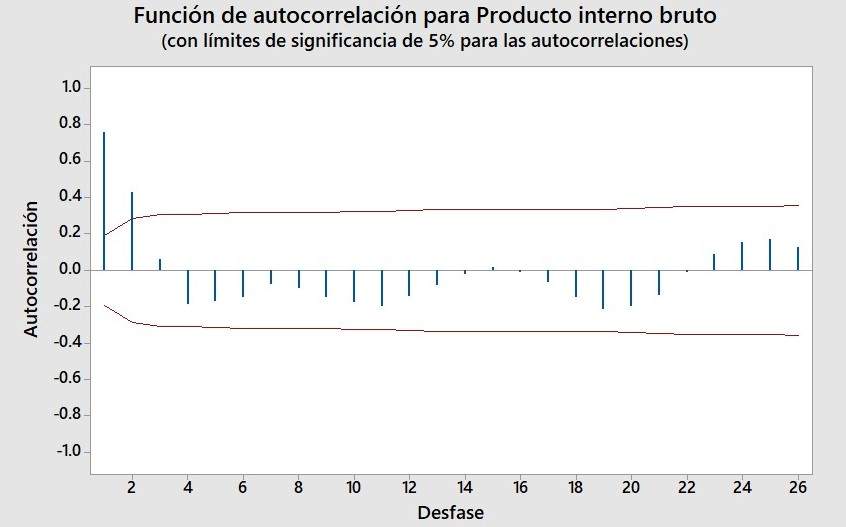
\includegraphics[width=0.7\textwidth]{7.jpg}
\caption{\label{fig:tesla}Matríz de autocorrelación.}
\end{figure}

\subsection{Modelo lineal}

El primer paso fue proponer un modelo general que nos incluya todas las variables para ver si estas son significativas o no en la descripción del PIB.\\

Dicho modelo quedó de la siguiente forma:

\begin{eqnarray}
PIB = \beta_0 + \beta_1 \log(fix) + \beta_2 \log(industrial) + \beta_3 \log(inverfij) + \beta_4 \log(consumo) + \nonumber\\
\beta_5 \log(balanzaex) + \beta_6 \log(balanzaimp) + \beta_7 lag(PIB)
\end{eqnarray}

La cual nos dio el siguiente análisis de varianza:
\newpage

\begin{figure}[h]
\centering
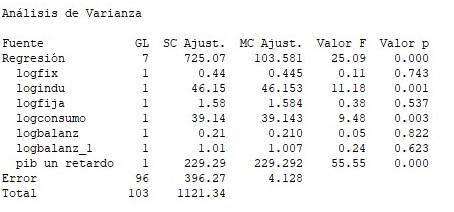
\includegraphics[width=0.7\textwidth]{8.jpg}
\caption{\label{fig:tesla}Análisis de la varianza.}
\end{figure}

Utilizando la prueba P para la significancia de las variables pudimos ver que solo 3 de ellas cumplen con ser estadísticamente significativas para nuestro modelo lo que nos dejó con un modelo de la siguiente forma:

\begin{equation}
    PIB = \beta_0 + \beta_1 \log(industrial) + \beta_2 \log(consumo) + \beta_3 lag(PIB) 
\end{equation}

A continuación, se hizo un análisis de la regresión lineal obtenida de dicho modelo:

\begin{figure}[h]
\centering
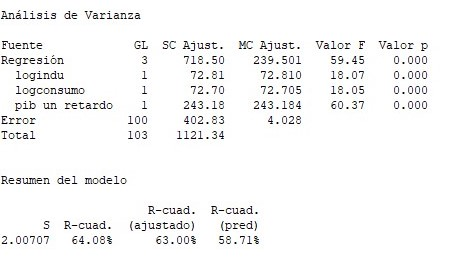
\includegraphics[width=0.7\textwidth]{9.jpg}
\caption{\label{fig:tesla}Resultados de la regresión.}
\end{figure}

Como fue de esperarse, se cumplió que las 3 variables son estadísticamente significativas bajo la prueba P. Por otro lado, este modelo nos dio una R-cuadrada de 64.08\% por lo cual podemos decir que es un modelo suficientemente robusto.

Así, la ecuación de nuestro modelo final es: 

\begin{equation}
    PIB = -61.6 + 72.9 \log(industrial) -41.6 \log(consumo) + 0.57 lag(PIB) 
\end{equation}

Cabe aclarar que, dado el ambiente de alta volatilidad, estos modelos no deben de ser utilizados para hacer pronósticos de más de uno o dos unidades en el futuro puesto que ello causaría una inflación en la varianza a tal medida que las estimaciones del modelo se harían poco precisas.

\newpage

\subsection{Pronostico del PIB utilizando el modelo propuesto}

Una manera de ver que tan bien calibrado es nuestro modelo es hacer predicciones sobre valores conocidos. Para ello hemos utilizado los datos de nuestro último periodo:

\begin{table}[h]
\centering
\begin{tabular}{l c r} 
%nùmero de columnas: 3
log industria & log consumo & lag PIB \\ \hline
2.00534 & 2.07042 & -0.3
\end{tabular}
\caption{\label{tab:tabla ejemplo}Valores en el último periodo observado.}
\end{table}

Lo cual nos da como resultado:

\begin{figure}[h]
\centering
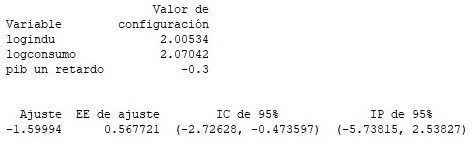
\includegraphics[width=0.7\textwidth]{10.jpg}
\caption{\label{fig:tesla}Resultados de la predicción.}
\end{figure}

Conocemos que bajo estos supuestos el valor del PIB fue de -0.5, el cual justamente está contenido en el intervalo de confianza de nuestra predicción, por ende, podemos asegurar que este modelo está bien calibrado.  De esta forma, nos permitimos estar seguros para realizar predicciones a futuro utilizando nuestro modelo propuesto.
\newline
Lamentablemente no hay datos oficiales de los indicadores que necesitamos para poder realizar la predicción. Sin embargo, podemos ver como estos indicadores se desarrollaron en situaciones similares como la crisis de 08-09 donde también existía una pandemia. Aunque no fue del alcance económico y social que se está mostrando actualmente, podemos darnos una idea a grandes rasgos comparando ambos escenarios.
\newline
\newline
Dicho el último punto, realizar una predicción de los datos basados en la especulación y haciendo uso de datos arbitrarios sería una irresponsabilidad de nuestra parte. Sin embargo, una vez liberados estos datos podemos utilizar este modelo para pronosticar el PIB. 
\newline
Cabe aclarar que, dado el ambiente de alta volatilidad, estos modelos no deben de ser utilizados para hacer pronósticos de más de uno o dos unidades en el futuro puesto que ello causaría una inflación en la varianza a tal medida que las estimaciones del modelo se harían poco precisas.

\section{Discusión}

Nuestro interés particular en este caso fue modelar el comportamiento del PIB mexicano con el factor COVID 19 influenciando los indicadores económicos; con el fin de observar el impacto de la pandemia actual en la economía de nuestro país, ya que la predicción no era nuestro punto clave por las razones que explicamos previamente en nuestro último punto del modelo. 
\newline
\newline
El resultado de la regresión nos dice que el PIB puede ser modelado como una relación lineal entre la actividad industrial, el consumo privado y el PIB en el periodo anterior.
\newline
\newline
La aparición de la nueva cepa de coronavirus hizo que México tomara medidas de distanciamiento social desde el mes de marzo por lo cual el sector comercial se vio directamente afectado. Resultando así en una desaceleración de la actividad económica industrial y mermando la capacidad de consumo de los ciudadanos. 
\newline
\newline
Tomando en cuenta la tendencia a la baja que ha venido mostrando el PIB en los últimos 3 trimestres del año pasado es claro que la expectativa para el primer trimestre del año sea negativa. Sumando a esto la falta de medidas contra cíclicas para reactivar los sectores de la economía que se encuentran en pausa, podemos especular que esta tendencia se mantendrá al menos para el segundo trimestre del 2020.

\subsection{Conclusión.}

El panorama creado por el COVID-19 ha hecho que los gobiernos inviertan desprevenidamente en el sector público de salud y en la seguridad social. La busqueda de estimular una economía en cuarentena los ha obligado a que se dobleguen y apliquen políticas dramaticas en orden de mitigar el impacto causado por la pandemia. 
\newline
\newline
En el caso de nuestro país, México, estas políticas han sido controversiales y han generado debate. Hay una fuerte tensión en el ámbito económico y, a través de los resultados encontrados en esta investigación, podemos ver los sectores que más incertidumbre están trayendo a la ecuación de medición y su relación con los demás sectores y con el COVID-19.
\newline
\newline
El ambiente no es favorecedor y no parece cambiar, hay una clara desaceleración en la economía del país y no parece que haya manera de cambiar la situación en 180 grados con las medidas implementadas actualmente.
\newline
\newline
Se requiere una serie de soluciones coordenadas para solventar el impacto que hay en la producción y el consumo para reactivar y acelerar la economía de México. La comunicación y transparencia es crucial.

\begin{thebibliography}{99}

\bibitem{Banxico1} Morales Y. (2020, febrero). Banxico baja rango del PIB para el 2020 ante debilidad económica. Recuperado de: https://www.eleconomista.com.mx/economia/Banxico-baja-rango-del-PIB-para-el-2020-ante-debilidad-economica-20200227-0031.html

\bibitem{Expansion1} (2020, febrero). El PIB de México descendió 0.1\% real durante 2019. Recuperado de: https://expansion.mx/economia/2020/06/01/pib-mexico-caera-8-y-dolar-llegara-23-pesos-analistas

\bibitem{Economista} Morales R. (2020, abril). México tendrá la peor caída del PIB por el Covid-19: OMC. Recuperado de: https://www.eleconomista.com.mx/empresas/Mexico-tendra-la-peor-caida-del-PIB-por-el-Covid-19-OMC-20200416-0044.htmll

\bibitem{Banxico2} (2020, mayo). Banxico advierte caída histórica de hasta 14\% del PIB: la recesión se prolongaría a 2021. Recuperado de: https://www.infobae.com/america/mexico/2020/05/05/banxico-advierte-caida-historica-en-la-actividad-economica-la-recesion-se-prolongara-hasta-2021/

\bibitem{Expansion2} Zavala J. (2020, junio). El PIB de México caerá \% y el dólar llegará a 23 pesos, prevén analistas. Recuperado de: https://expansion.mx/economia/2020/06/01/pib-mexico-caera-8-y-dolar-llegara-23-pesos-analistass

\bibitem{Forbes} Coll F. (2020, mayo). Análisis COVID-19: México registra su mayor contracción económica desde 2009. https://www.forbes.com.mx/analisis-covid-19-mexico-registra-su-mayor-contraccion-economica-desde-2009/

\end{thebibliography}

\end{document}